\chapter{光子軌道、林德勒空間與史瓦西黑洞內部}

牛頓力學中的點質量與史瓦西黑洞，起初採用相同的理想化假設：所有產生引力的質量都集中在中心。然而，兩者的中心意義截然不同。在牛頓力學中，粒子只要有些微角動量，就會錯過中心。在黑洞中，粒子一旦越過視界，就無法避開奇點。要理解這項差異，我們將依序探討圓軌道、光子球，最後再介紹視界附近的一組新座標。

\section{無法避開的中心}

真實的牛頓物質永遠不會成為數學上的點。壓力、材料強度及其他作用力都會抵抗壓縮。即使仍把點質量當作理想化模型，下落的粒子也很少會撞上它。嚴格徑向的軌跡可以抵達\(r=0\)，但再微小的橫向速度也會帶來角動量。離心勢壘接著會使粒子繞過中心。

廣義相對論改變了這個結論。足夠緻密的天體可以形成黑洞，而黑洞內部無法像牛頓力學那樣繞過中心逃逸。原因比「力更強」來得深刻：在視界內，\(r\)減小是指向未來的方向。我們將逐步推導出這個結論，而不是預先假定它成立。

\begin{classroomqa}
\audiencequestion{牛頓力學中難以擊中中心，是否只是因為把兩個物體都理想化成點？}
\lecturerresponse{點的理想化是這項比較的一部分，但並非差異的全部。在牛頓力學中，任何非零角動量都會使軌道繞過那個點。在相對論的黑洞內部，奇點位於每一條下落類時軌跡的未來；角向運動無法讓粒子逃脫。
\lecturetimestamp{00:04:52--00:05:13}}
\end{classroomqa}

\section{視界與奇點}

我們暫且把史瓦西幾何視為已知：
\begin{equation}
d\tau^{2}
=
\left(1-\frac{2MG}{r}\right)dt^{2}
-
\frac{dr^{2}}{1-\frac{2MG}{r}}
-
r^{2}d\Omega^{2}.
\label{eq:l6-schwarzschild}
\end{equation}
選出這個度規的場方程稍後再談。眼前的任務是理解這個度規所描述的物理。

單位球面上的度規可以寫成
\begin{equation}
d\Omega^{2}
=d\vartheta^{2}+\cos^{2}\vartheta\,d\phi^{2}
\label{eq:l6-angular-metric}
\end{equation}
其中\(\vartheta\)是從赤道面量起的緯度。若改用較常見、從軸量起的極角，餘弦就會變成正弦。由於球對稱性，任何軌道都可以放在一個固定平面內，因此接下來的計算只會用到一個角座標。

\begin{figure}[htbp]
\centering
\includegraphics[width=0.88\textwidth]{lecture_06_figure_01.png}
\caption{史瓦西度規，以及曲面\(r=2MG\)的柱狀時空示意圖。中心線是\(r=0\)；紅色柱面表示史瓦西座標中的視界。}
\lectureframe{00:09:45}
\end{figure}

遠離引力源時，\(2MG/r\)很小，式~\eqref{eq:l6-schwarzschild}趨近於球座標下的閔可夫斯基度規。有兩個半徑特別值得注意：
\begin{equation}
r=2MG,
\qquad
r=0.
\end{equation}
兩者不可混為一談。在\(r=2MG\)處，\(dt^{2}\)的係數為零，而\(dr^{2}\)的係數發散；史瓦西座標系在此變得奇異，但曲率仍有限。相較之下，在\(r=0\)處，曲率不變量發散。潮汐場會無限制地沿徑向拉伸延展物體、沿橫向擠壓物體。這是物理上的奇點，而非座標缺陷。

\subsection{計量下落的兩種方式}

對於位於視界外的靜止時鐘，
\begin{equation}
d\tau
=
\sqrt{1-\frac{2MG}{r}}\,dt.
\label{eq:l6-static-clock}
\end{equation}
當\(r\)很大時，\(d\tau\simeq dt\)。在視界附近，若時鐘維持在固定的\(r\)，它的固有時間相對於遠處記錄的史瓦西時間會推進得非常緩慢。

同一組座標描述徑向下落時，需要讓\(t\)取無窮大，才能抵達\(r=2MG\)。但下落者自身經歷的固有時間有限，這兩種說法並不矛盾。下落者攜帶的時鐘測量沿其世界線流逝的固有時間。這個時鐘可以是機械鐘、由米尺兩端的鏡子構成的光鐘、一次心跳，或大腦中一連串物理過程。這些都不會測量遠處的座標時間\(t\)。近視界圖將呈現這兩種計時方式的差異。

\section{從固有時作用量推導圓周運動}

回到下落問題之前，先來解決另一個問題：有質量粒子或光子在什麼條件下能繞黑洞運行？計算從所有自由運動相對論粒子都適用的作用量原理開始，
\begin{equation}
S=-m\int d\tau.
\label{eq:l6-particle-action}
\end{equation}
光線會受地球彎曲，但地球的引力場遠不足以讓光線形成封閉軌道。地球的史瓦西半徑只有約一公分。必須把整個地球壓縮到大致這個尺度，也就是小堅果般的大小，強場問題才會變得切題。

令\(c=1\)，將運動限制在赤道面內，並定義
\begin{equation}
F(r)=1-\frac{2MG}{r},
\qquad
G(r)=\frac{1}{F(r)}.
\label{eq:l6-fg}
\end{equation}
以座標時間\(t\)作為參數，可得
\begin{equation}
d\tau
=dt\sqrt{F-G\dot r^{\,2}-r^{2}\dot\theta^{\,2}},
\end{equation}
因此
\begin{equation}
\mathcal L
=
-m\sqrt{F-G\dot r^{\,2}-r^{2}\dot\theta^{\,2}}.
\label{eq:l6-lagrangian}
\end{equation}
因子\(m\)使作用量具有通常的能量乘時間量綱。

\begin{figure}[htbp]
\centering
\includegraphics[width=0.76\textwidth]{lecture_06_figure_02.png}
\caption{黑板上正在推導平方根形式的粒子拉格朗日量。完整表示式見式~\eqref{eq:l6-lagrangian}。}
\lectureframe{00:31:53}
\end{figure}

對任意廣義座標\(q\)，
\begin{equation}
p_q=\frac{\partial\mathcal L}{\partial\dot q}.
\end{equation}
我們以\(\mathcal L\)表示拉格朗日量，以\(L\)表示角動量。令
\begin{equation}
\Delta=F-G\dot r^{\,2}-r^{2}\dot\theta^{\,2},
\end{equation}
兩個共軛動量為
\begin{align}
L=p_\theta
&=\frac{mr^{2}\dot\theta}{\sqrt{\Delta}},
\label{eq:l6-angular-momentum}\\
p_r
&=\frac{mG\dot r}{\sqrt{\Delta}}.
\label{eq:l6-radial-momentum}
\end{align}
由於徑向座標出現在拉格朗日量中，徑向動量並不守恆。拉格朗日量中沒有角度\(\theta\)，因此\(L\)守恆。

\(t\)也沒有顯含於\(\mathcal L\)中，因此哈密頓量守恆：
\begin{align}
E=H
&=p_r\dot r+L\dot\theta-\mathcal L \\
&=\frac{mG\dot r^{\,2}}{\sqrt{\Delta}}
  +\frac{mr^{2}\dot\theta^{\,2}}{\sqrt{\Delta}}
  +m\sqrt{\Delta} \\
&=\frac{mF}{\sqrt{\Delta}}.
\label{eq:l6-energy-general}
\end{align}
這是力學中常見的脈絡：原理給出作用量，計算得到動量，而對稱性再將計算結果連結回能量守恆與角動量守恆。當然，也可以立刻求解所有尤拉--拉格朗日方程；不過，旋轉對稱性與時間平移對稱性所帶來的守恆量，能省去許多計算。

\subsection{圓軌道的能量}

對圓軌道而言，
\begin{equation}
\dot r=0.
\end{equation}
引入單位質量的角動量，
\begin{equation}
\lambda=\frac{L}{m}.
\end{equation}
式~\eqref{eq:l6-angular-momentum}與\eqref{eq:l6-energy-general}變為
\begin{align}
\lambda
&=\frac{r^{2}\dot\theta}
{\sqrt{F-r^{2}\dot\theta^{\,2}}},
\label{eq:l6-lambda-circular}\\
E
&=\frac{mF}{\sqrt{F-r^{2}\dot\theta^{\,2}}}.
\label{eq:l6-energy-circular-first}
\end{align}

\begin{figure}[htbp]
\centering
\includegraphics[width=0.82\textwidth]{lecture_06_figure_04.png}
\caption{史瓦西時空中圓周運動的約化角動量與能量。先利用角動量方程，從能量式中消去\(\dot\theta\)。}
\lectureframe{00:39:14}
\end{figure}

將式~\eqref{eq:l6-lambda-circular}平方並解出角速度，可得
\begin{equation}
\dot\theta^{\,2}
=
\frac{\lambda^{2}F}
{r^{2}\left(r^{2}+\lambda^{2}\right)}.
\label{eq:l6-angular-speed}
\end{equation}
代入式~\eqref{eq:l6-energy-circular-first}後，能量便只取決於所考慮的半徑與固定的角動量：
\begin{equation}
E(r,\lambda)
=m\sqrt{F(r)}\,\frac{\sqrt{r^{2}+\lambda^{2}}}{r}.
\label{eq:l6-circular-energy}
\end{equation}

課堂上停下來與牛頓力學作比較。一般圓軌道的角頻率與切向速率會隨半徑增加而降低，但角動量還包含一個半徑因子。因此，不能只憑角速度判斷\(L\)如何變化。相對論公式明確保留了這些因子。

\section{光子的圓軌道}

光子雖然靜止質量為零，仍具有能量與動量，因此取式~\eqref{eq:l6-circular-energy}的無質量極限時必須小心。如果\(m\)在\(\lambda\)固定時趨近於零，\(L=m\lambda\)也會趨近於零。應改為令
\begin{equation}
m\longrightarrow0,
\qquad
\lambda\longrightarrow\infty,
\qquad
L=m\lambda\ \text{fixed}.
\label{eq:l6-massless-limit}
\end{equation}
此時\(\lambda^{2}\)項佔主導，光子的能量變為
\begin{equation}
E_\gamma(r;L)
=L\,\frac{\sqrt{1-\frac{2MG}{r}}}{r}.
\label{eq:l6-photon-energy}
\end{equation}
因子\(L\)乘上整個徑向函數。它會影響能量的尺度，但不影響圓軌道的半徑。

\begin{figure}[htbp]
\centering
\includegraphics[width=0.88\textwidth]{lecture_06_figure_05.png}
\caption{光子能量中的徑向因子。在視界處它為零，半徑增大時也會趨近於零，且在兩者之間有一個極大值。}
\lectureframe{00:50:50}
\end{figure}

固定\(L\)時，徑向平衡要求函數有駐點：
\begin{equation}
\frac{d}{dr}
\left[
\frac{\sqrt{1-\frac{2MG}{r}}}{r}
\right]=0.
\end{equation}
對它微分，
\begin{equation}
-\frac{\sqrt{1-\frac{2MG}{r}}}{r^{2}}
+
\frac{MG}
{r^{3}\sqrt{1-\frac{2MG}{r}}}
=0,
\end{equation}
因此
\begin{equation}
r=3MG.
\label{eq:l6-photon-sphere}
\end{equation}
這個半徑是史瓦西半徑的1.5倍，通常稱為光子球。

這個駐點是極大值，因此光子的圓軌道不穩定。光子若恰好位於\(3MG\)，便會停留在那裡；但任何微小的徑向位移，最終都會使它離開這個極大值。略在光子球之外的光線，可以掃過很大的角度，甚至在逃逸前繞黑洞多圈。略在光子球之內的近切向光線，也可能繞行數圈，接著穿過視界落入黑洞。

\begin{figure}[htbp]
\centering
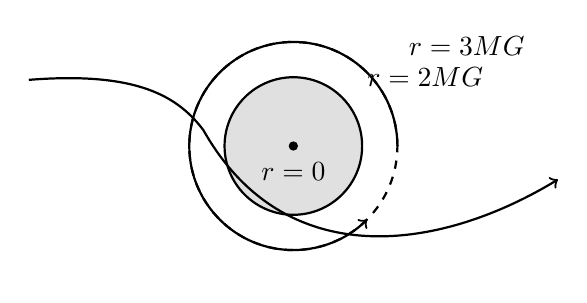
\begin{tikzpicture}[scale=1.12]
\fill[black!12] (0,0) circle (0.78);
\draw[thick] (0,0) circle (0.78);
\draw[dashed,thick] (0,0) circle (1.18);
\fill (0,0) circle (1.5pt);
\draw[->,thick] (1.18,0) arc (0:315:1.18);
\draw[->,thick] (-3.0,0.75)
  .. controls (-1.75,0.85) and (-1.30,0.55) .. (-1.02,0.18)
  .. controls (-0.10,-1.45) and (1.65,-1.20) .. (3.0,-0.38);
\node[right] at (0.73,0.78) {\(r=2MG\)};
\node[right] at (1.20,1.13) {\(r=3MG\)};
\node[below] at (0,-0.08) {\(r=0\)};
\end{tikzpicture}
\caption{視界、光子球與一條大幅偏折的光線。光線若任意接近不穩定圓軌道，就能在逃逸或向內落入前累積任意大的偏折角。}
\end{figure}

\begin{classroomqa}
\audiencequestion{為什麼要固定角動量？它與光子的頻率及入射軌跡有何關係？}
\lecturerresponse{每條光線都帶有相對於黑洞守恆的角動量。光子的頻率決定線動量的大小，而光線相對於中心的偏移也有助於決定\(L\)。若不要求圓軌道，半徑與角動量可以各自選定。若要求光子沿圓軌道運動，兩者便會連結到唯一的半徑\(3MG\)；式~\eqref{eq:l6-photon-energy}中的因式分解顯示，這個半徑與\(L\)的大小無關。
\lecturetimestamp{00:54:43--00:57:02}}
\end{classroomqa}

\begin{classroomqa}
\audiencequestion{為什麼能量的極大值可以決定軌道？}
\lecturerresponse{固定\(L\)並消去角向運動後，剩下的函數便扮演有效徑向能量的角色。駐點代表徑向平衡；若駐點是極小值，平衡便是穩定的。此處是極大值，因此對應不穩定的圓軌道。稱它既是平衡又是不穩定，並不矛盾。
\lecturetimestamp{00:57:51--00:58:54}}
\end{classroomqa}

有質量粒子可以在\(3MG\)之外沿類時圓軌道運動，不過最靠近光子球的那些軌道是不穩定的。無質量粒子則只有在\(3MG\)處才能沿圓軌道運動。在光子球內，切向運動的光子會向內落入；運動速度更慢的物體也不會更有機會維持這種軌道。這裡談的是角向運動。在視界外，即使起始半徑小於\(3MG\)，方向足夠朝外的光線仍然可以逃逸。

\section{黑洞如何改變影像}

光子球說明了黑洞並非只是在原本不變的天空上貼了一塊暗盤。背景天體發出的光可以沿多條路徑抵達觀測者：一條光線從黑洞一側通過，另一條從另一側通過，還有其他光線可能繞黑洞一圈或多圈。因此，影像可能出現位移、重影、光環，還有一串因額外繞行而形成、愈來愈細微也愈來愈暗的影像，數量無窮。實際影像雖然複雜，成因已包含在這條不穩定軌道之中。

當光源、透鏡與觀測者大致排列成一直線時，影像可能形成愛因斯坦環。自然界中確實觀測到引力透鏡環。要得到完整的黑洞影像，必須針對許多初始方向積分零測地線，這項計算很適合交由電腦處理。

\begin{classroomqa}
\audiencequestion{這個光學邊界指的是光子球還是視界？}
\lecturerresponse{兩者扮演不同角色。位於\(2MG\)的視界是因果邊界：任何指向未來的訊號都無法從內部逃出。位於\(3MG\)的光子球則影響切向運動與強引力透鏡效應。在這兩個半徑之間，朝外的徑向光線可以逃逸，切向光線則會落入。介於兩者之間的方向可能使光線先繞行，再逃逸或被捕獲。
\lecturetimestamp{01:02:47--01:03:40}}
\end{classroomqa}

\begin{classroomqa}
\audiencequestion{一般的光線路徑能不能實際算出來，而不只是畫個示意圖？}
\lecturerresponse{可以。將零條件代入測地線方程或尤拉--拉格朗日方程，再依選定的初始條件積分即可。這些方程的概念並不新，但光線追蹤的代數計算相當繁瑣，因此實際繪製影像時通常會採用數值方法。
\lecturetimestamp{01:03:48--01:04:27}}
\end{classroomqa}

\begin{classroomqa}
\audiencequestion{若直接使用尤拉--拉格朗日方程，圓軌道的計算會不會更困難？}
\lecturerresponse{結果會相同。無論採用哪種方法，作用量都是恰當的出發點；但循環座標會揭示守恆的能量與角動量。先利用這些守恆量，是推導圓軌道條件較直接的做法。
\lecturetimestamp{01:04:33--01:05:49}}
\end{classroomqa}

\section{近視界度規就是林德勒空間}

現在回到視界。史瓦西度規的係數在此處看似發散或消失，穿越視界時它們的正負號還會互換。然而，下落觀測者經過這個表面時，不會遇到發散的局部曲率。等效原理說明了這兩件事如何能同時成立。

先從二維閔可夫斯基時空開始：
\begin{equation}
d\tau^{2}=dT^{2}-dX^{2}.
\end{equation}
在右側林德勒楔形區定義
\begin{equation}
X=\rho\cosh\omega,
\qquad
T=\rho\sinh\omega.
\label{eq:l6-rindler-map}
\end{equation}
\(\rho\)固定的曲線滿足
\begin{equation}
X^{2}-T^{2}=\rho^{2},
\end{equation}
因此它們是雙曲線，也就是等加速度觀測者的世界線。將式~\eqref{eq:l6-rindler-map}代入平直時空的度規，可得
\begin{equation}
d\tau^{2}
=\rho^{2}d\omega^{2}-d\rho^{2}.
\label{eq:l6-rindler-metric}
\end{equation}
現在令
\begin{equation}
\rho^{2}=4\xi,
\qquad
\omega=\frac{t}{2}.
\label{eq:l6-rindler-rescale}
\end{equation}
由於\(d\rho^{2}=d\xi^{2}/\xi\)，式~\eqref{eq:l6-rindler-metric}便成為
\begin{equation}
d\tau^{2}
=\xi\,dt^{2}-\frac{d\xi^{2}}{\xi}.
\label{eq:l6-xi-metric}
\end{equation}

\begin{classroomqa}
\audiencequestion{角向座標或橫向座標去哪裡了？}
\lecturerresponse{它們只是暫時省略了。我們正在考察包含穿越視界行為的局部\(t\)-\(r\)平面。兩個橫向方向仍然規則，可以再加回來；它們不會改變目前分析的座標奇異性。
\lecturetimestamp{01:16:27--01:16:47}}
\end{classroomqa}

為了與史瓦西度規比較，選用\(2MG=1\)的單位。式~\eqref{eq:l6-schwarzschild}的徑向部分為
\begin{equation}
d\tau^{2}
=
\frac{r-1}{r}\,dt^{2}
-
\frac{r}{r-1}\,dr^{2}.
\end{equation}
非常接近\(r=1\)時，分子中的小量\(r-1\)必須保留；其他原本無關緊要的\(r\)因子則可近似為1。因此
\begin{equation}
d\tau^{2}
\simeq
(r-1)\,dt^{2}
-
\frac{dr^{2}}{r-1}.
\end{equation}
令
\begin{equation}
\xi=r-1,
\end{equation}
這正是式~\eqref{eq:l6-xi-metric}。在視界附近，史瓦西幾何局部上就是平直時空的林德勒描述。

\begin{classroomqa}
\audiencequestion{如果底層時空是平直的，這些怎麼會是加速座標？}
\lecturerresponse{加速度屬於觀測者，不一定源自曲率。固定在\(\rho\)的世界線，在閔可夫斯基時空中是等加速度運動。同樣地，黑洞附近維持固定半徑的觀測者，必須受到支撐以抵抗自由落體。完整的史瓦西時空雖然是彎曲的，等效原理仍使局部描述相符。
\lecturetimestamp{01:22:19--01:24:06}}
\end{classroomqa}

\section{穿越林德勒視界}

右楔形區的公式只適用於\(\xi>0\)：
\begin{equation}
X=2\sqrt{\xi}\cosh\frac{t}{2},
\qquad
T=2\sqrt{\xi}\sinh\frac{t}{2}.
\label{eq:l6-rindler-outside}
\end{equation}
曲面\(\xi=0\)就是零線\(X=T\)。若要延伸到未來楔形區，令
\begin{equation}
\zeta=-\xi>0
\end{equation}
並交換雙曲函數的角色：
\begin{equation}
T=2\sqrt{\zeta}\cosh\frac{t}{2},
\qquad
X=2\sqrt{\zeta}\sinh\frac{t}{2}.
\label{eq:l6-rindler-inside}
\end{equation}
度規仍為
\begin{equation}
d\tau^{2}
=\xi\,dt^{2}-\frac{d\xi^{2}}{\xi},
\end{equation}
但在\(\xi<0\)時，\(dt^{2}\)的係數為負，\(d\xi^{2}\)的係數為正。座標\(\xi\)，也就是史瓦西徑向方向，已變成類時；\(t\)則變成類空。

\begin{figure}[htbp]
\centering
\includegraphics[width=0.88\textwidth]{lecture_06_figure_06.png}
\caption{林德勒楔形區、其零邊界，以及從\(\xi>0\)延伸至\(\xi<0\)的情形。黑板上還記下了\(\rho^{2}=4\xi\)與\(\omega=t/2\)。}
\lectureframe{01:29:40}
\end{figure}

\begin{classroomqa}
\audiencequestion{這張座標圖中有些曲線看起來比光還快嗎？}
\lecturerresponse{座標網格線不一定代表物質物體的世界線。網格線的座標斜率可能看似超光速，但這不違反因果律。物理光線仍沿零線傳播，物理粒子仍位於當地光錐之內。
\lecturetimestamp{01:28:44--01:29:08}}
\end{classroomqa}

繼續深入史瓦西黑洞內部，最終會抵達\(r=0\)。這個邊界是類空的，因此將它描述為一段時間，比描述為一個地點更恰當：黑洞內部每一條指向未來的類時或零軌跡都會抵達那裡。人可以繞過一個地點，卻無法繞過自己的未來。

\begin{classroomqa}
\audiencequestion{圖中的曲線能否直接穿過\(r=0\)延伸到負\(r\)，而\(r=0\)仍然是中心嗎？}
\lecturerresponse{座標圖或許會讓人想把一條線延長，但經典的史瓦西解在曲率奇點處終止。\(r=0\)仍可稱為中心，但這是個非常特殊的中心：在黑洞內部，它是類空的未來邊界。不存在能穿過它、通往負半徑區域的規則通道。
\lecturetimestamp{01:32:16--01:34:06}}
\end{classroomqa}

\begin{classroomqa}
\audiencequestion{林德勒圖中的對角線是類光的嗎？下落者能在加速時間的有限值處進入嗎？}
\lecturerresponse{是的，楔形區的邊界是零線。自由落體世界線會在一個普通的有限事件、經過有限固有時間後穿越這條線。加速座標\(t\)，或等價地\(\omega\)，在外部固定\(\rho\)的描述中沒有上下界；趨於無限的是座標標記，而非穿越事件本身。
\lecturetimestamp{01:34:26--01:35:03}}
\end{classroomqa}

\section{外側的 Alice 與下落的 Bob}

讓 Alice 留在外側的固定半徑處，並由外力支撐以抵抗引力；Bob 則自由下落。在視界附近，Alice 沿著類似林德勒雙曲線的世界線運動。她的固定\(t\)切片愈來愈密集地逼近零邊界。對 Bob 世界線上的每一個事件，只要 Alice 賦予的\(t\)有限，該事件就位於視界之外；因此她從不會以有限的史瓦西時間標記 Bob 穿越視界的事件。

Bob 攜帶一只固有時間時鐘。他的軌跡在時鐘所量得的有限時間內穿越零線。穿越時，局部不會發生任何發散現象。視界在全局上具有決定性，在局部卻是平常的。

\begin{figure}[htbp]
\centering
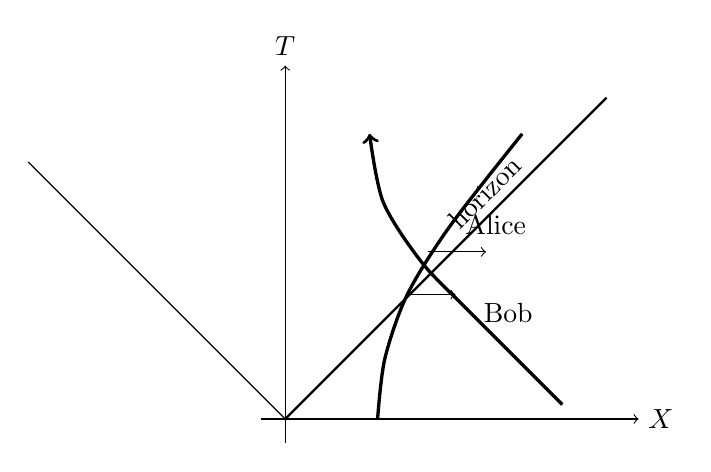
\begin{tikzpicture}[scale=1.02]
\draw[->] (-0.3,0) -- (4.4,0) node[right] {\(X\)};
\draw[->] (0,-0.3) -- (0,4.4) node[above] {\(T\)};
\draw[thick] (0,0) -- (4.0,4.0);
\draw[thin] (0,0) -- (-3.2,3.2);
\node[rotate=45,above] at (2.65,2.65) {horizon};
\draw[very thick]
  plot[smooth] coordinates {(1.15,0.0) (1.24,0.75) (1.52,1.55)
  (2.05,2.40) (2.95,3.55)};
\node[right] at (2.12,2.42) {Alice};
\draw[very thick,->]
  plot[smooth] coordinates {(3.45,0.18) (2.85,0.78) (2.25,1.38)
  (1.70,1.95) (1.22,2.70) (1.05,3.55)};
\node[right] at (2.35,1.32) {Bob};
\draw[->] (1.52,1.55) -- (2.12,1.55);
\draw[->] (1.78,2.08) -- (2.50,2.08);
\end{tikzpicture}
\caption{Alice 在外側加速運動的世界線，以及 Bob 自由下落的世界線。Alice 的座標切片逼近視界；Bob 則在有限固有時間內穿越視界。}
\end{figure}

\begin{classroomqa}
\audiencequestion{Bob 回頭看 Alice 時會看到什麼？穿越視界後，他的時鐘又會如何？}
\lecturerresponse{Bob 會看到 Alice 帶著維持在外側所需的加速度逐漸遠離，但他在穿越視界時不會看到任何奇異事件。Alice 可以被支撐在固定半徑處；也可以考慮她沿軌道運動的另一種設定。Bob 的時鐘會繼續正常測量他的固有時間\(\tau\)。在內部，說徑向座標是類時的，是在描述因果幾何；這不會真的把他的腕錶變成米尺。他的世界線最終會在\(r=0\)終止。
\lecturetimestamp{01:39:51--01:44:45}}
\end{classroomqa}

現在我們認出這條零線就是視界本身，而不只是座標係數出現異常的某一點。在視界外，有一族徑向光線向外傳播；在視界內，未來光錐的兩個方向都通往更小的\(r\)。每一條指向未來的有質量粒子軌跡都必須留在這兩個零方向之間，因此終將抵達奇點。

\section{訊號、紅移與正在形成的視界}

假設坍縮中的物質發出一串規則的光脈衝。遠處的觀測者接收到後續脈衝的時間間隔會愈來愈長。脈衝頻率會從可見光波段移向紅外線、微波、無線電波，波長還會繼續增長。在理想化的經典計算中，外部觀測者仍可將愈來愈晚抵達的訊號與接近視界的物質聯繫起來；但在實際上，光源很快就會變得紅移且微弱到無法探測。

\begin{classroomqa}
\audiencequestion{坍縮期間，外部觀測者是否會看到所有物質就此凍結在視界上？}
\lecturerresponse{以史瓦西時間描述時，坍縮物質的表面會漸近地逼近視界，看起來愈來愈像凍結不動。實際上觀測到的是光訊號；這些訊號會愈來愈延遲、紅移，也愈來愈微弱。這種座標描述並不表示下落物質經歷了無限長的固有時間。
\lecturetimestamp{01:47:06--01:48:11}}
\end{classroomqa}

\begin{classroomqa}
\audiencequestion{足夠晚才開始觀測的人，能否還原下落的完整歷程？}
\lecturerresponse{只能依靠已發出且成功抵達觀測者的訊號。接續而來的脈衝彼此間隔愈來愈長，也愈來愈紅移。靈敏度無限高的理想觀測者，可以追蹤經典訊號，直到波長變得任意長；實際的觀測者則會看著天體逐漸暗去、消失。
\lecturetimestamp{01:48:13--01:52:00}}
\end{classroomqa}

\begin{classroomqa}
\audiencequestion{說奇點是一段時間而非一個地點，確切來說是什麼意思？}
\lecturerresponse{\(r=0\)這個面是類空的。進入視界後，每一條指向未來的類時或零曲線都會在那裡終止。空間中的一個位置可以改走別條路來避開；但沿著指向未來的世界線前進，就無法避開未來邊界。
\lecturetimestamp{01:52:02--01:53:10}}
\end{classroomqa}

那麼，如果外部觀測者永遠看不到物質穿越視界，黑洞如何形成或增大質量？考慮一個正在坍縮的球殼。全局視界並不是預先存在、停留在固定半徑的物質表面。它從中心開始向外擴展，並在黑洞區域形成時與坍縮中的球殼相遇。外部的史瓦西描述仍顯示球殼漸近地逼近最終視界。完整的時空圖像，以及如何從全局角度定位視界，將在下一講討論。

\begin{figure}[htbp]
\centering
\includegraphics[width=0.90\textwidth]{lecture_06_figure_07.png}
\caption{坍縮中的球殼，以及從中心向外擴展、與球殼相遇的視界。這幅圖預覽了下一講將深入探討的全局坍縮幾何。}
\lectureframe{01:57:25}
\end{figure}

\begin{classroomqa}
\audiencequestion{如果外部座標時間中沒有任何東西穿越視界，黑洞如何形成或增長？}
\lecturerresponse{這個問題把座標描述與全局描述混為一談。坍縮物質會在有限固有時間內抵達相關區域，而事件視界則由整個時空的因果結構決定。在球殼圖像中，視界從中心開始向外擴展，與球殼相遇。外部觀測者看到的延遲且紅移的景象，與這個全局視界仍然一致。
\lecturetimestamp{01:53:11--01:57:34}}
\end{classroomqa}

\section{兩個球面之間的逃逸方向}

視界與光子球將光線的情形區分開來。在半徑
\begin{equation}
2MG<r<3MG,
\end{equation}
處，徑向向外的光線可以逃逸至無窮遠；切向光線則不能，會向內落入。兩種方向之間存在一個逃逸錐。愈接近視界，逃逸錐就愈集中在徑向向外的方向。越過視界後，逃逸錐便完全閉合。

\begin{classroomqa}
\audiencequestion{位於視界與光子球之間的光源，能向外傳送任何訊號嗎？}
\lecturerresponse{可以。只要發射事件發生在\(2MG\)之外，方向足夠接近徑向向外的零測地線就能逃逸。光子在\(3MG\)內作角向運動會向內落入，這並不表示徑向向外的光線也不能逃逸。結果取決於發射方向；光源愈接近視界，容許向外逃逸的角錐就愈窄。
\lecturetimestamp{01:57:34--01:59:48}}
\end{classroomqa}

\begin{classroomqa}
\audiencequestion{從外側入射的光線能否穿過光子球內部、轉向後再度射出？}
\lecturerresponse{對於這裡討論的零測地線，無法如此。若光線在某處轉向，該處的徑向速度必須為零；也就是說，光線會在低於\(3MG\)的半徑處瞬間呈切向，而此處的角向軌跡會向內落入，無法再向外轉回。不過，原本就在兩個球面之間的光源，仍可在穿越視界前發出方向足夠接近徑向向外的光線。
\lecturetimestamp{01:59:49--02:01:27}}
\end{classroomqa}

最後一個問題刻意保留較多未定之處。設想 Alice 和 Bob 都被固定在視界外相同的半徑處。附近的觀測者顯然可以互相傳送訊號。如果他們沿球面相距很遠，直接的零測地線路徑及其可達角度範圍上限，就需要明確計算測地線才能確定。課堂提出一條間接路徑：將訊息幾乎沿徑向向外傳送到較安全半徑處的中繼站，在那裡轉送至另一側，再向內傳回。另一種方式是讓向外拋出的物體或訊號折返。這些路徑說明，切向圓軌道無法存在，並不代表外部觀測者之間完全無法通訊。

\begin{classroomqa}
\audiencequestion{兩個觀測者懸停在相同的近視界半徑處，能否繞著黑洞互相通訊？}
\lecturerresponse{就局部而言，可以。對於相距很遠或位於直徑兩端的觀測者，講座中並未計算直接路徑的極限，因此不應將其說成定理。討論一開始將角度方向上的測地線問題留待解答，接著指出，訊號可以沿近乎徑向的方向向外傳送，在較大半徑處經由中繼繞至另一側，再傳回來。愈接近視界，直接傳送訊號所適用的角度範圍就愈窄；但只要仍在視界之外，向外傳送的路徑就仍然可行。
\lecturetimestamp{02:01:29--02:04:17}}
\end{classroomqa}

接下來要以坍縮天體的全域幾何取代這些近視界的示意圖，並精確探討事件視界如何增長。